\documentclass[12pt,a4paper]{article}
\usepackage[utf8]{inputenc}
\usepackage[T2A]{fontenc}
\usepackage{graphicx}
\usepackage{color}
\usepackage{url}
\usepackage[unicode]{hyperref}
\usepackage{biblatex}
\renewcommand{\contentsname}{Садржај}

\usepackage{tabularx}
\usepackage{multicol}
%\usepackage[english,serbian]{babel}

\definecolor{mypink1}{rgb}{0.858, 0.188, 0.478}
\hypersetup{colorlinks, citecolor=red, linkcolor=mypink1, urlcolor=blue}

\bibliography{spisak} 

\begin{document}

\title{\textbf{Мартин Фаулер \\(софтверски инжењер)}\\ \small{Семинарски рад у овиру курса\\ \href{http://www.itkomunikacija.matf.bg.ac.rs/TehnickoINaucnoPisanje.html}{Техничко и научно писање}\\\href{http://www.matf.bg.ac.rs/}{Математички факултет}}}
\author{Марија Ристић, Нина Докмановић\\marija230700@gmail.com\\ninadokmanovic2.nd@gmail.com}
\date{9.~новембар 2019}

\maketitle
\tableofcontents
\newpage

\section{{Увод}}
\label{sec:uvod}
\textbf{Мартин Фаулер} (рођен 1963) је британски програмер, аутор и међународни јавни говорник о софтверском развоју, специјализован за oбјектно-оријентисане анализе и дизајн , UML језик, обрасце и методологију развоја агилних софтвера, укључујући екстремно програмирање. \\Његова књига, објављена 1999. године, учинила је популарним процес реструктурирања постојећег рачунарског кода\cite{k_1}. Године 2004. увео је модел презентација, архитектонски образац.\cite{k_2}
\section{{Биографија}}
\label{sec:biografija}
Рођен је и одрастао је у Волсолу, у Енглеској, где је похађао гимназију Краљица Марија. Дипломирао је на Лондонском универзитетском колеџу 1986. Године 1994. преселио се у Сједињене Америчке државе, где живи у близини Бостона, Масачусетс у предграђу Мелроуз\cite{sajt}.\\
Фаулер је почео рад на софтверима почетком 1980-их. Ван универзитета, 1986. године, почео је да ради на развоју софтвера за \emph{Coopers and Lybrand} све до 1991.\cite{k_3} године. Године 2000. придружио се \emph{ThoughtWorks}, компанији за системску интеграцију и консултантско предузеће\cite{sajt}, где ради као главни научник.\cite{sajt_2}\\
Фаулер је написао девет књига на тему развоја софтвера (више у одељку Књиге). Члан је Агилне aлијансе и помогао је у креирању Манифеста за развој агилних софтвера 2001. године, заједно са 16 сарадника потписника.\cite{sajt_3} Одржава блики, комбинација блога и вики-ја. Учинио је популарнијим термин убризгавање зависности као облик инверзије контроле. \cite{sajt_4, knjiga}

\begin{tabular}{|r|l|}\hline
    \multicolumn{2}{|c|}{\textbf{Мартин Фаулер}}\\
    \multicolumn{2}{|c|}{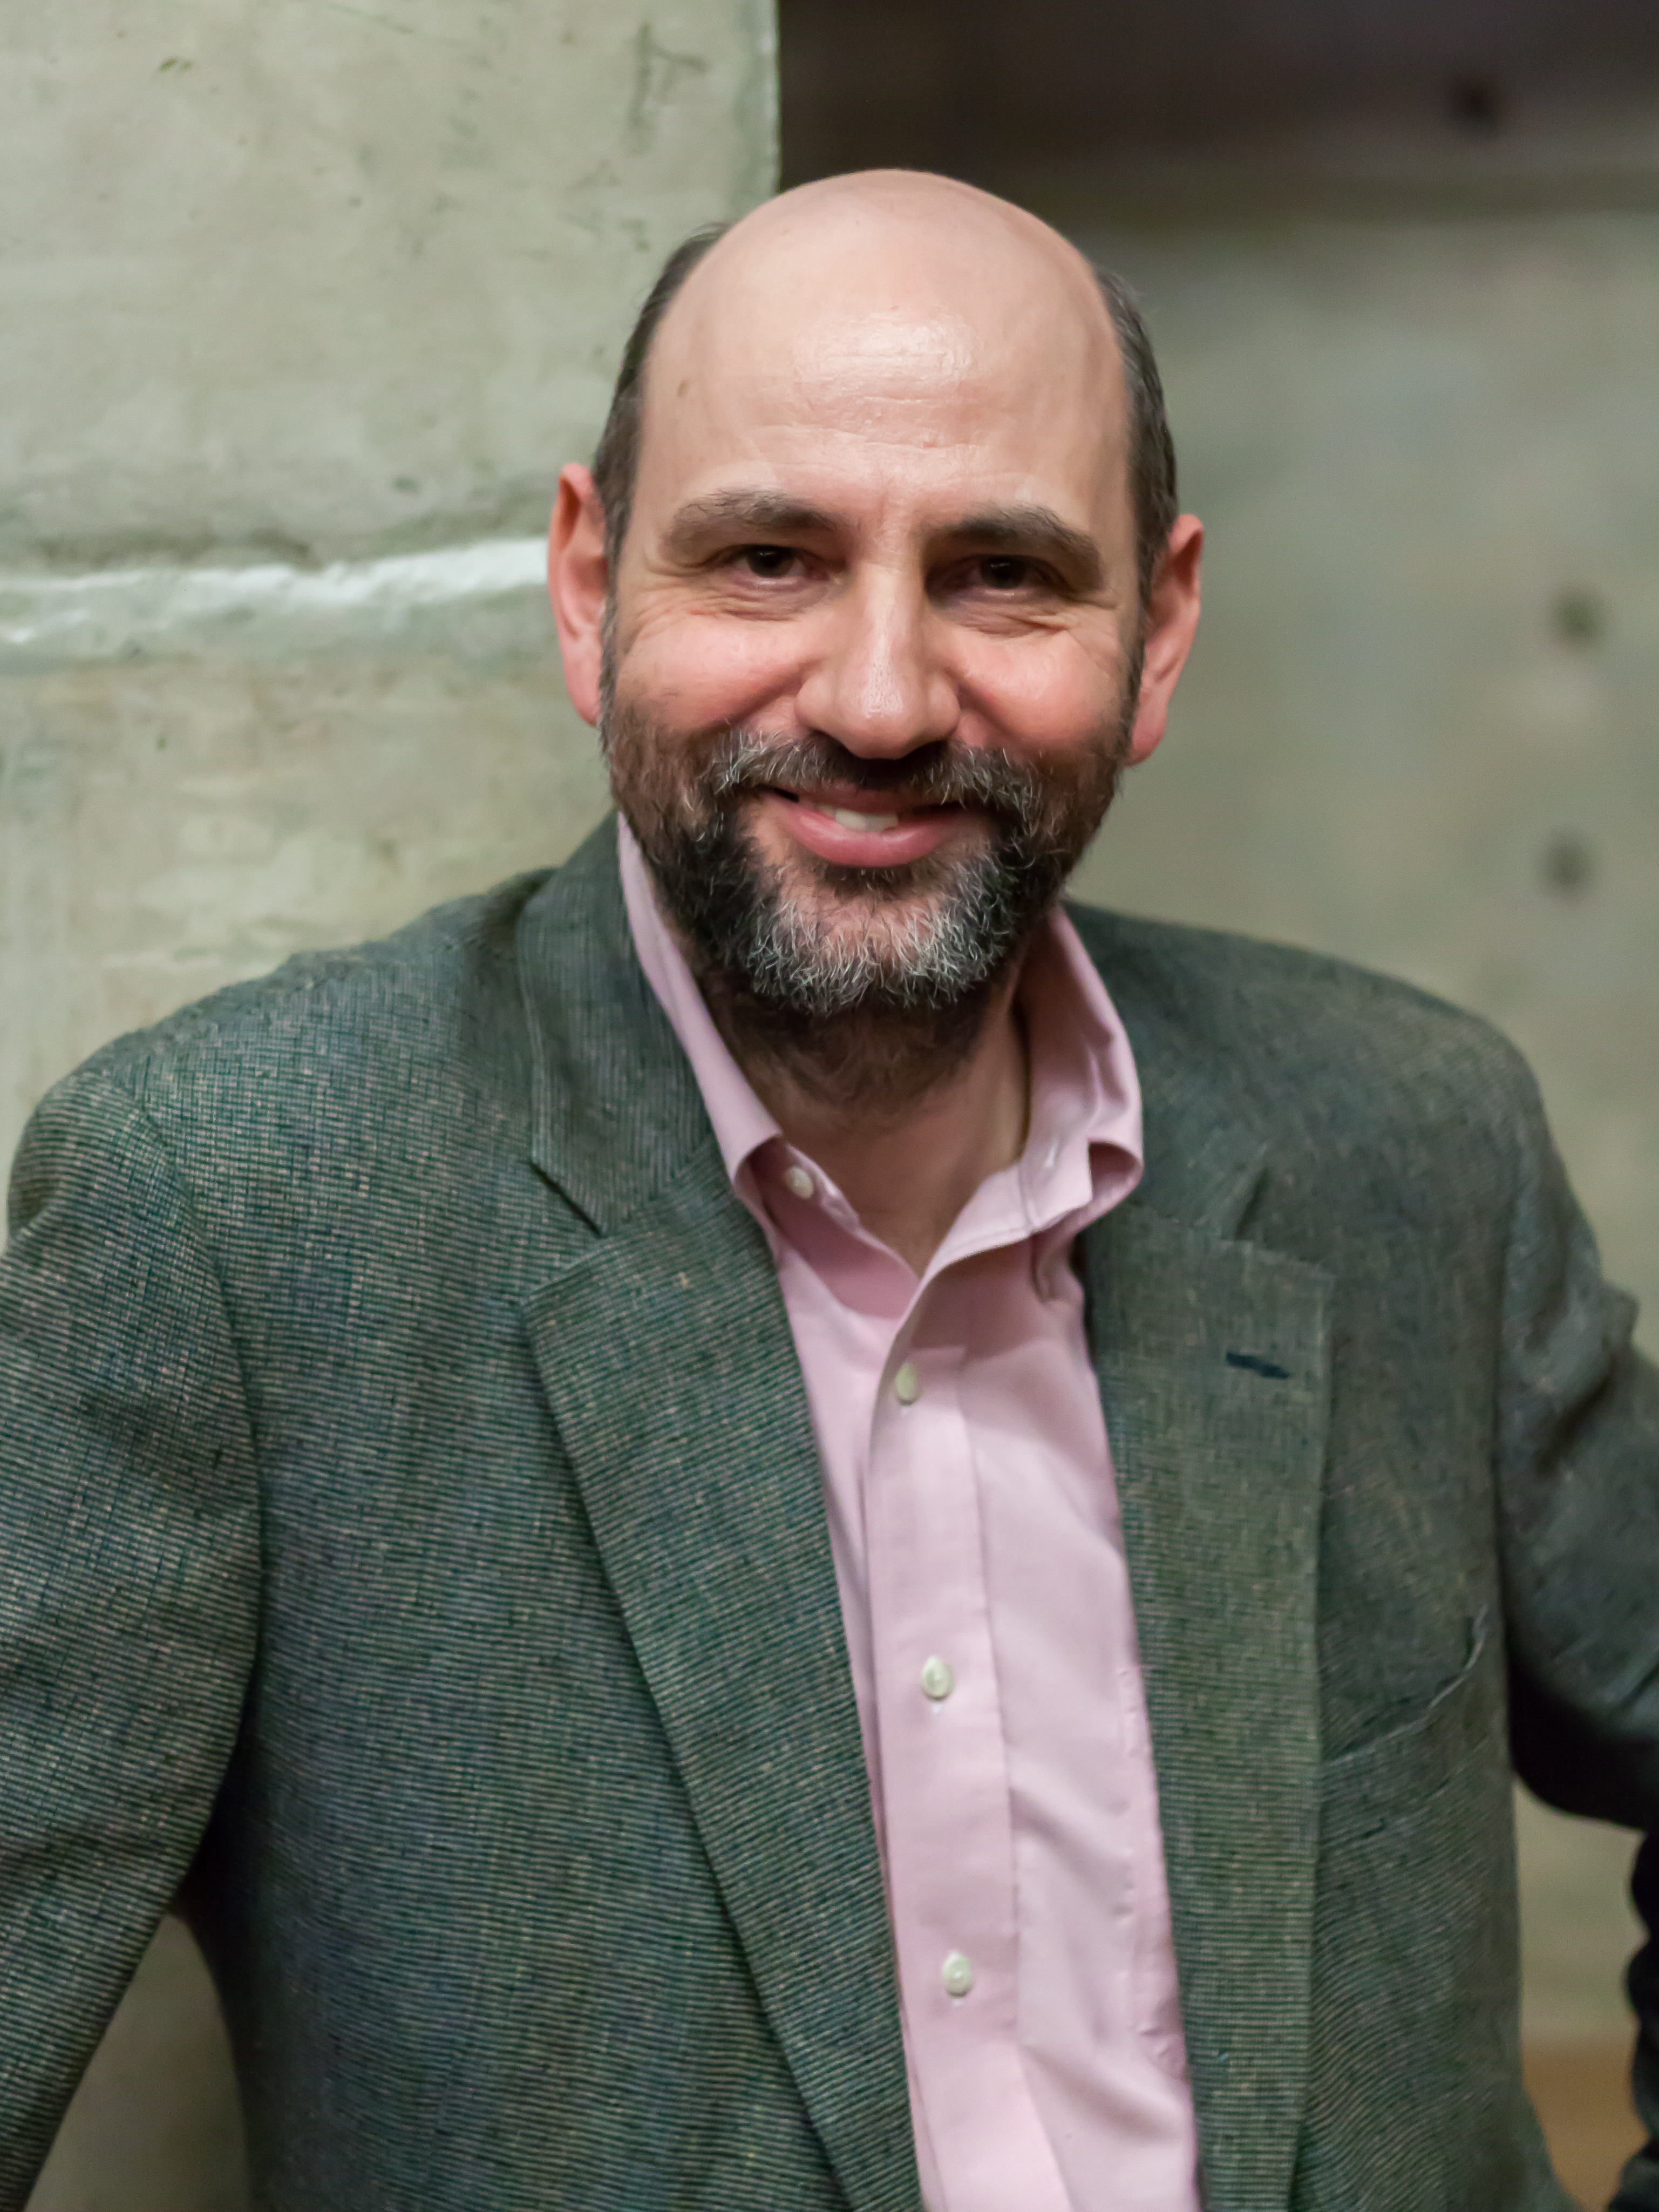
\includegraphics[width=0.45\textwidth, height=80mm]{Martin_Fowler.png}} \\

    \textbf{Датум рођења} & 1963 \\ \cline{2-2}
    \textbf{Место рођења} & Волсол, \\
     &  Енглеска \\ \cline{2-2}
     \textbf{Пребивалиште} & Мелроуз, \\
      & Масачусетс \\ \cline{2-2}
     \textbf{Образовање} & Лондонски универзитетски колеџ \\ \cline{2-2}
     & Софтверски инжењер, \\
     \textbf{ Занимање} & аутор, \\
      & јавни говорник \\ \cline{2-2}
     \textbf{Послодавац} & \emph{ThoughtWorks} \\ \cline{2-2}
     \textbf{Веб-сајт}	& 	martinfowler.com \\ \hline
\end{tabular}
\newpage

\section{{Списак књига}}
\begin{itemize}
    \item 1996. Обрасци анализе: Модели објеката који се могу поново користити (енгл. \emph{Analysis Patterns: Reusable Object Models}). Едисон-Весли
    \item 1997. UML укратко: кратак водич за стандардни језик моделовањa објеката (енгл. \emph{UML Distilled: A Brief Guide to the Standard Object Modeling Language}). Едисон-Весли
    \item 1999. ,,Рефакторисање је процес промене софтверског система на такав начин да не мења екстерно понашање кода, али ипак побољшава 1његову унутрашњу структуру. "- Мартин Фаулер у књизи Рефакторисање: Побољшање дизајна постојећег кода (енгл. \emph{Refactoring: Improving the Design of Existing Code}) , са Кентом Беком, Џоном Брантом, Вилијамом Опдикеом и Доном Робертсом. Едисон-Весли
    \item 2000. Планирање екстремног програмирања (енгл. \emph{Planning Extreme Programming}). Са Кентом Беком. Eдисон-Весли
    \item 2002. Обрасци архитектуре примене предузећа (енгл. \emph{Patterns of Enterprise Application Architecture}). Уз Давида Рајса, Метјуа Фоимела, Едварда Хајта, Роберта Миа и Рендија Стафорда. Едисон-Весли
    \item 2010. Обласно-специфичан језик (енгл. \emph{Domain-Specific Languages}). Са Ребеком Парсонс. Едисон-Весли
    \item 2012.\emph{NoSQL Distilled: A Brief Guide to the Emerging World of Polyglot Persistence}. Са Прамодом Садалагеом. Едисон-Весли
    \item 2013. Рефакторисање: Рубиново издање (енгл.\emph{Refactoring: Ruby Edition}). Уз Кента Бека, Шејна Харвија и Џеја Филдса. Едисон-Весли
    \item 2018. Рефакторисање: Побољшање дизајна постојећег кода, друго издање (енгл. \emph{Refactoring: Improving the Design of Existing Code, Second Edition}). Кент Бек и Мартин Фаулер. Едисон-Весли
\end{itemize}

\newpage

\addcontentsline{toc}{section}{Литература}
\appendix

\printbibliography[title=Литература]

\section{Спољашње везе}
\begin{itemize}
    \item \href{https://martinfowler.com/}{Званична страница} 
    \item \href{https://www.artima.com/intv/martin.html}{Интервју са Мартином Фаулером} 
\end{itemize}
\begin{table}
\begin{center}
\begin{tabular}{|m{3cm}|m{11cm}|} \hline
     \multicolumn{2}{|c|}{\textbf{Софтверски инжењеринг}} \\ \hline
     \textbf{Области} & Програмирање Анализа захтева Одржавање софтвера Софтверски дизајн Софтверско распоређивање Софтверско тестирање Системска анализа Формалне методе \\ \hline
     \textbf{Концепти} & Моделирање података Предузећа архитектуре Функционална спецификација Моделирање језика Парадигме програмирања Софтвер Софтверска археологија Софтверска архитектура Конфигурацијски менаџмент софтвера Методологија развоја софтвера Развојни циклус софтвера Квалитет софтвера Софтверско осигурање квалитета Софтверска верификација и валидација Структурна анализа \\ \hline
     \textbf{Оријентација} & Агилни Аспектно-оријентисан Објектно-оријентисано Онтологија Сервис оријентација SDLC \\ \hline
     \textbf{Модели} & {
     \begin{tabular}{m{1.8cm}|m{8.5cm}}
          Развојни & Agile EUP Извршни UML Постепен модел Итеративни модел Мoдел прототипа RAD UP Скрам Спирални модел V-модел Водопад модел XP \\ \hline
          Друго & SPICE CMMI Модел података ER модел Функционални модел Информациони модел Метамоделирање Објектни модел Системски модел Преглед модел \\ \hline
          Језици & IDEF UML SysML \\
     \end{tabular}
     } \\ \hline
     \textbf{Софтверски инжењери} & Кент Бек Грејди Бух Фред Брукс Бери Боем Вард Канингем Том Демарко Едсгер Дајкстра Мартин Фаулер Тони Хор Маргарет Хефилд Хамилтон Грејс Хопер Лојс Хејбт Ватс Хамфри Мајкл А. Џексон Ивар Јакобсон Стивен Мелор Бертранд Мејер Алан Кеј Дејвид Парнас Винстон В. Ројс Џејмс Рамбо Никлаус Вирт Едвард Јордан Виктор Базили \\ \hline
     \textbf{Повезане области} & Информатика Рачунарски инжењеринг Управљање пројектима Управљање ризиком Системски инжењеринг \\ \hline
\end{tabular}
\end{center}
\end{table}

\end{document}
